%*****************************************
\chapter{Implementation}\label{ch:implementation}
%*****************************************

\FloatBarrier
\section{Extension structure}

We describe the overall structure of the extension and the C++ library. We also describe how the extension is loaded and initialised.

\subsection{Overview}

    Aside from some boilerplate Firefox extension code and the JavaScrypt Stego! library (see section XXX) the main body of the application is made up of five components, shown on Figure \ref{uml:component}:

    \begin{figure}[tb]
        \begin{center}
                \includegraphics{gfx/component.1}
            \caption{UML component diagram for the extension.}
            \label{uml:component}
        \end{center}
    \end{figure}
    
    \begin{sdesc}
     
    \item[Toolbar XUL] \hfill \\ The toolbar XUL defines the toolbar interface using the Mozilla XML User Interface Language (XUL). The component is loaded as part of the browser chrome when Firefox is started and is responsible for loading the JavaScript components.
    
    \item[Page interception] \hfill \\ {\tt pagecept} contains the HTML parser for extracting prospective decryption targets and inserting UI controls. Actual target processors and control event handlers are defined in {\tt efb}. This layer of abstraction means updates due to changes in the Facebook web site are isolated to this component. Component re-use (e.g. in an extension for another browser) is also fascillitated. 

    \item[Main extension component] \hfill \\ {\tt efb} defines the handlers for the toolbar and integrated UI controls. It contains handlers for decryption events and contains the plaintext cache data structures. It also contains callback handlers for asynchronous {\tt faceapi} function calls. During the login process {\tt efb} attaches the {\tt pagecept} HTML parser to page loading events and initialises the C++ module, binding the native methods to JavaScript wrapper functions.
    
    \item[Facebook API layer] \hfill \\ {\tt faceapi} is a layer of abstraction between {\tt efb} and the Facebook platform. {\tt faceapi} contains code for Graph API read/write queries as well as for the workaround solutions detailed in section XXX.

    \item[C++ Module] \hfill \\ Primarily contains codec algorithms and cryptographic functions.
    
    \end{sdesc}
    

\subsection{C++ module structure}

    The C++ module contains a library instance which implements the {\tt IeFBLib} interface. The exposed behaviors of this libary are wrapped appropriately so they may be called from the JavaScript module.
    
    The library itself utilises four polymorphic sub-components:
    
    \begin{itemize}
    
        \item {\tt ICrypto} contains cryptographic algorithms.
        \item {\tt IFec} contains error correction algorithms.
        \item {\tt IStringCodec} contains a UTF-8 encoder/decoder.
        \item {\tt IConduitImage} contains JPEG-immune image coding algorithms.
    
    \end{itemize}
    
    This design fascillitates future extension and possible run time composition of different sub-components - though currently the concrete implementations are chosen at design time. \footnote{Since only one set of components currently provides a feasible solution, see evaluation section XXX} The first three components are instantiated upon initialisation of the module. The last ({\tt IConduitImage}) is generated whenever an image is encoded or decoded. Since C++ does not natively define interfaces we use an abstract base classe with all pure virtual methods and a virtual destructor to disable polymorphic destruction \cite{interfaces}. 
    
    The library is built around the abstract factory pattern described in \cite{dpatterns}. This allows us to encapsulate groups of complimentary sub-components since some interdepenence exists between sub-components. \footnote{For example, the minimum size of the encryption header can't exceed the maximum capacity of the conduit image.} Figure \ref{uml:lib-classes} outlines the pattern structure with an example concrete subclass {\tt HaarWTConduitImage}.
    
    \begin{figure}[tb]
        \begin{center}
                \includegraphics{gfx/lib.1}
            \caption{UML class diagrams for the library and its sub-components.}
            \label{uml:lib-classes}
        \end{center}
    \end{figure}
    
    
\subsection{Initialisation}

Firefox loads the toolbar XUL as part of the chrome when the browser is started. The XUL then loads the javascript components which define handlers for the toolbar controls. The extension is initialised when either the start button or generate identity button is clicked. {\tt efb} harvests the Facebook ID from a browser cookie (assuming the user is logged in to Facebook) and uses it to define the working directory. The C++ library will then be instantiated and the {\tt pacecept} handler attached to page load events.


\FloatBarrier
\section{Integrating with the Facebook UI}

The {\tt pagecept} module checks if web pages are from the Facebook domain. If they are, it parses the HTML and attempts to insert additional UI controls and also retrieve and process any ciphered content automatically. 


\subsection{Inserting submission controls}

There are four types of submission control, each of which may appear in multiple places within a single page. These are for general posts (status updates and wall posts) comments, private messages and image uploads. Each control is assosciated with an input field. Finding control-field pairs involves several complex regex queries which we will not discuss in detail.

Once a pair has been identified we generate an alternative encrypted submission control and place it beside the normal one. A handler is generated assosciated with the input field. For images this process is slightly different - a check box is added and the handler to the normal control modified.

The submission handler causes a friend selector window to appear, loaded with any friends whose public keys are stored on disk. Elements within the control are populated with the user's names and profile pictures by performing queries through {\tt faceapi}. Optionally, Encrypted Facebook will check if local public keys are up to date with online keys. The user is given the option of updating an out of date key, and is informed of the tradeoff between vulnerability to middleperson attacks and potential non-availability.

On submission, the selected list of friends and the input from the input fields are gathered and processed by {\tt efb}. The submission process is detailed in section XXX.


\subsection{Retrieving content}

Regexes are used to locate and filter possible decryption targets. For text these will be enclosed by special start and end sequences. Images can be identified by their filename as Graph API objects. In either case we can not be certain and so filtering is a "best effort" approach. Malicious user could easily create fake text tags, and most Graph API images won't be encrypted. The decryption process is designed to fail gracefully as early as possible if this turns out to be the case. Currently, since all images are 720x720 pixels this predicate is used as a filter. The case for uploading variable sized images and its effect on filtering are discussed in section XXX.

Once a list of target Facebook IDs has been generated and filtered, it is processed. Each ID is checked to see if it has an entry in the cache. If not, an entry is created and a XmlHttpRequest triggered though {\tt efb}. A handler is attached to the requst so that on completion, the cache can be updated appropriately. If an entry exists then several actions may be appropriate. If a valid plaintext exists in the cache this is used. The entry may also be marked as in progress in which case a loading message is substituted. If a previous attempt failed then the target can be ignored.


    
\FloatBarrier
\section{Text submission}

We consider the process by which a plaintext message, given a list of recipients, is transformed to a steganography encoded tag which points to the ciphered message stored online as a note. This tag can then be used in place of the plaintext.

    \begin{figure}[tb]
        \begin{center}
                \begin{tikzpicture}[
box/.style={
    draw, font={\footnotesize \bfseries},
    minimum width=3cm, minimum height=1cm, text centered, thick, black!100},
lab/.style={
    right,
    font={\scriptsize},
    text width=5cm},
lab2/.style={
    align=right,
    below left,
    font={\scriptsize},
    text width=3cm} 
]

% nodes
\node (start) at (0,0) {};
\node[box] (recieve) [below=0.5cm of start] {Recieve};
\node[box] (encrypt) [below=1cm of recieve] {Encrypt};
\node[box] (encode) [below=1cm of encrypt] {UTF-8 Encode};
\node[box] (return) [below=1cm of encode] {Return};
\node[box] (submit) [below=1cm of return] {Submit};
\node[box] (stego) [below=1cm of submit] {Stego! Encode};
\node (end) [below=0.5cm of stego] {};

% descr
%\node[lab] at (recieve.east) () {Prepend empty space for header};
%\node[lab] at (encrypt.east) () {No size increase, header writen to empty space};
%\node[lab] at (encode.east) () {Unpredectible output size. Between 1-4 $\times$ $\lceil \frac{input}{2} %\rceil$ possibly plus 4-byte padding flag prepended};
%\node[lab] at (return.east) () {Null terminal appended};

% types
%\node[lab2, above left] at (recieve.north) () {char* $\times$ \\ char*};
%\node[lab2] at (recieve.south) () {vector<byte> $\times$ \\ vector<FacebookId>};
%\node[lab2] at (encrypt.south) () {vector<byte>};
%\node[lab2] at (encode.south) () {string};
%\node[lab2] at (return.south) () {char*};

\draw [decorate,decoration={brace,amplitude=5pt}]
    ($(recieve.north east)+(0.2,0)$)  -- ($(return.south east)+(0.2,0)$);
\node[lab] at ($(encrypt.south east) + (0.3,-0.5)$) () {C++ module};

%arrows
\draw [->,>=stealth, thick] (start.south) -- (recieve.north);
\draw [->,>=stealth, thick] (recieve.south) -- (encrypt.north);
\draw [->,>=stealth, thick] (encrypt.south) -- (encode.north);
\draw [->,>=stealth, thick] (encode.south) -- (return.north);
\draw [->,>=stealth, thick] (return.south) -- (submit.north);
\draw [->,>=stealth, thick] (submit.south) -- (stego.north);
\draw [->,>=stealth, thick] (stego.south) -- (end.north);



\end{tikzpicture}
            \caption{Encoding process for submitting text.}
            \label{tikz:text}
        \end{center}
    \end{figure}



The string is passed to the C++ library, encrypted then encoded in a UTF-8 based format suitable for Facebook. The result is returned to the JavaScript module, submitted and a tag generated from the resultant object ID using steganography. We describe each step of this process in detail.

\subsection{Encryption}

    \begin{figure}[tb]
        \begin{center}
                \includegraphics{gfx/crypto.1}
            \caption{UML class diagrams for the cryptography component.}
            \label{uml:crypto}
        \end{center}
    \end{figure}
    
Currently the only implementation for cryptographic functions is based on the Botan library using RSA and AES. The Botan library is encaspulated in a class with template parameters {\tt (N, M)} which determine the length (in bytes) of the AES session key and RSA public key, respectively.The class is designed so that a class with certain key sizes can be defined simply by specifying these paratameters.
    
    \begin{table}[tb]
        \begin{center}
                \begin{tabular}{|+l|^l|}
                    \hline
                    \rowstyle{\bfseries}%
                    Description & Size (bytes) \\ \hline
                    \hline
                    Length tag & 2\\ \hline
                    Initialisation vector & 16 \\ \hline
                    Facebook ID & 8 \\ \hline
                    Session key & {\it <pub-key size>} \\ \hline
                    \multicolumn{2}{c}{$\vdots$} \\ \hline
                    Facebook ID & 8 \\ \hline
                    Session key & {\it <pub-key size>} \\ \hline                    
                \end{tabular}
            \caption{Structure of the encryption header.}
            \label{tab:crypto}
        \end{center}
    \end{table}
    
The input string is converted to a byte vector containing enough free space at the begining for the encryption header (the size of the crypto header can be calculated in advance based on the recipient list so that encryption can be performed in place) along with a recipient list of Facebook IDs. The output is the ciphered message with the encryption header prepended.

Table \ref{tab:crypto} describes the format of the crypto header generated as part of the broadcast encryption scheme. Note that the public key size determines the cipher block size and therefore the storage requirements for the encyrpted session key - regardless of the actual session key length itself.

The Botan SecureVector data structure is used to intermediately store all cryptographic keys, preventing key material being swapped to disk. A random IV and session key is generated for every message using Botan, which is supposedly reasonably random \cite{XXX}. After encryption, all seeds, key material and IVs are disposed of securely.


\FloatBarrier
\subsection{String coding}

The input is a byte vector of random bytes from the encryption stage. Each 16-bit (2 bytes) code is mapped on to a valid UTF-8 character - a variable length sequence of 1 to 5 bytes. Odd numbered input is padded and a otherwise unused character sequence prepended to indicate this. The mapping is based on the mapping from Unicode code points to UTF-8 chars, with two distinctions.

\begin{itemize}

    \item Each 16-bit input is shifted by an offset of 0xB0 before being mapped to a character. This avoids problem symbol characters which will be escaped by the Facebook sanitization process (< and > for example).
    
    \item Unicode code points XXX-XXX are surrogate pair characters and are illegal if used in isolation. Inputs which map to these characters (after being offset) are bit-shifted left by one place.
    
\end{itemize}


Note that this means some of the resulting code points are outside the BMP (Basic Multilingual Plane) but are still well defined as UTF-8 characters and supported by Facebook.

After adding a null terminal the final string can be returned to the JavaScript calling function.


\FloatBarrier
\subsection{Submission as a note}

The final string is submitted as a note to Facebook via {\tt faceapi} passing the relevant handlers from {\tt efb}. On completion the Facebook Graph API object ID is parsed from the XmlHttpRequest response and encoded using the steganography functions provided by the JavaScrypt Stego! library. Start and end tags are added and the final text is ready to be used in place of the cleartext, as described in section XXX.



\FloatBarrier
\section{Image submission}

We now describe the process by which an image, stored locally, is encryped and encoded in a temporary image file ready to be uploaded. The C++ library is passed the input and output file paths and returns 0 on success.

Initially the image data is loaded from disk as a byte vector (leaving room for the encryption header) and encrypted exactly as described in section XXX. Error correcting codes are then added. Finally, a conduit image object is created, written to, and saved to disk. We describe the last two stages in detail.

    \begin{figure}[tb]
        \begin{center}
                \begin{tikzpicture}[
box/.style={
    draw, font={\footnotesize \bfseries},
    minimum width=3cm, text width=3cm, minimum height=1cm, text centered, thick, black!100},
lab/.style={
    right,
    font={\scriptsize},
    text width=5cm},
lab2/.style={
    align=right,
    below left,
    font={\scriptsize},
    text width=3cm} 
]

% nodes
\node (start) at (0,0) {};
\node[box] (recieve) [below=0.5cm of start] {Load from disk};
\node[box] (encrypt) [below=1cm of recieve] {Encrypt};
\node[box] (encode) [below=1cm of encrypt] {FEC Encode};
\node[box] (return) [below=1cm of encode] {Image Encode};
\node[box] (submit) [below=1cm of return] {Save to disk};
\node (end) [below=0.5cm of submit] {};

% descr
%\node[lab] at (recieve.east) () {Prepend empty space for header};
%\node[lab] at (encrypt.east) () {No size increase, header writen to empty space};
%\node[lab] at (encode.east) () {Unpredectible output size. Between 1-4 $\times$ $\lceil \frac{input}{2} %\rceil$ possibly plus 4-byte padding flag prepended};
%\node[lab] at (return.east) () {Null terminal appended};

% types
%\node[lab2, above left] at (recieve.north) () {char* $\times$ \\ char*};
%\node[lab2] at (recieve.south) () {vector<byte> $\times$ \\ vector<FacebookId>};
%\node[lab2] at (encrypt.south) () {vector<byte>};
%\node[lab2] at (encode.south) () {string};
%\node[lab2] at (return.south) () {char*};

%arrows
\draw [->,>=stealth, thick] (start.south) -- (recieve.north);
\draw [->,>=stealth, thick] (recieve.south) -- (encrypt.north);
\draw [->,>=stealth, thick] (encrypt.south) -- (encode.north);
\draw [->,>=stealth, thick] (encode.south) -- (return.north);
\draw [->,>=stealth, thick] (return.south) -- (submit.north);
\draw [->,>=stealth, thick] (submit.south) -- (end.north);



\end{tikzpicture}
            \caption{Encoding process for submitting an image.}
            \label{tikz:text}
        \end{center}
    \end{figure}


\FloatBarrier
\subsection{Error correction}

Currently the only implementations are based on the Shifra library using Reed Solomon codes. The bulk of the Shifra library is encapsulated in an abstract base class and two template specialisation subclasses implementing codes rates of (15,9) and (255,223) (see Figure \ref{uml:fec}).


    \begin{figure}[tb]
        \begin{center}
                \includegraphics{gfx/fec.1}
            \caption{UML class diagrams for the forward error correction libary component.}
            \label{uml:fec}
        \end{center}
    \end{figure}

The FEC algorithms have a fixed block size. In order to avoid excess padding bytes or addition length tags, we use a scheme inspired by ciphertext stealing used in crytography \cite{XXX}. The FEC codes are appended to the data bytes so that, provided there are enough blocks, any last partial block will be padded out automatically.


\FloatBarrier
\subsection{Conduit image class hierarchy}

Images are encoded by generating an instance of IConduitImage through the abstract factory, writing data to it, then saving out to disk. The CImg class (from the CImg library) is used as a base class since it supports opening and saving various image formats, manipulating pixels and colour space transforms.

    \begin{figure}[tbp]
        \begin{center}
                \includegraphics{gfx/img.1}
            \caption{UML class diagrams for the conduit image implementation.}
            \label{uml:img-classes}
        \end{center}
    \end{figure}
    

\FloatBarrier
\subsection{Read/write buffering}

All current implementations are derived from the abstract class {\tt BufferedConduitImage } which implements read and write buffers. This allows us to group single byte read/write requests together, which is nessescary for certain implementations. The Haar wavelet method, for example, stores 3-bytes at a time in 8x8 pixel blocks.

The variables {\tt rhead} and {\tt whead} determine the current position of the read and write heads, or equivalently the number of bytes written or read since creation. {\tt block\_size} is set upon instantiation through the constructor and is the smallest integer number of bytes that can be read/written at once.

Any subclass of {\tt BufferedConduitImage } must provide a function {\tt getBlockCoords }. This maps the position of the read/write heads to block coordinates within the image.  Subclasses must also implement {\tt encodeInBlock } and {\tt decodeFromBlock } for writing {\tt block\_size} bytes to and from a block given the block coordinates.

This class also contains gray code translation functions, since they are used by all descendant classes and their definitions are too small to justify a class of their own.

\begin{table}[tbph]
    \begin{center}
            
            \begin{tabular}{+l ^l ^l ^l}
                \rowstyle{\bfseries}%
                Class & \parbox[t][][t]{12ex}{\raggedright Dimensions (pixels)} & \parbox[t][][t]{12ex}{\raggedright Block size (bytes)} & \parbox[t][][t]{12ex}{\raggedright Grey codes (bits)} \\
                \midrule
                Haar WT & 8 $\times$ 8 & 3 & 6 \\
                3-bit Scaling & 3 $\times$ 2 & 3 & 3\\
                4-bit Scaling & 2 $\times$ 1 & 1 & 4
            \end{tabular}
            
        \caption{Comparison of blocks for each concrete subclass}
        \label{tab:blocks}
    \end{center}
\end{table}
    
\FloatBarrier
\subsection{Haar wavelet transform}

The {\tt HaarWTConduitImage} uses blocks of 8x8 pixels, with a block size of 3-bytes. Two passes of the 2D Haar wavelet transform are performed on a single block. 6 bits are written to the high order bits of each of the four 8-bit approximation coeffients. The low order bits are masked of based on experimental results, and as suggested in \cite{XXX}. The inverse transform is then performed to output greyscale pixel values.

\begin{figure}
\begin{center}

    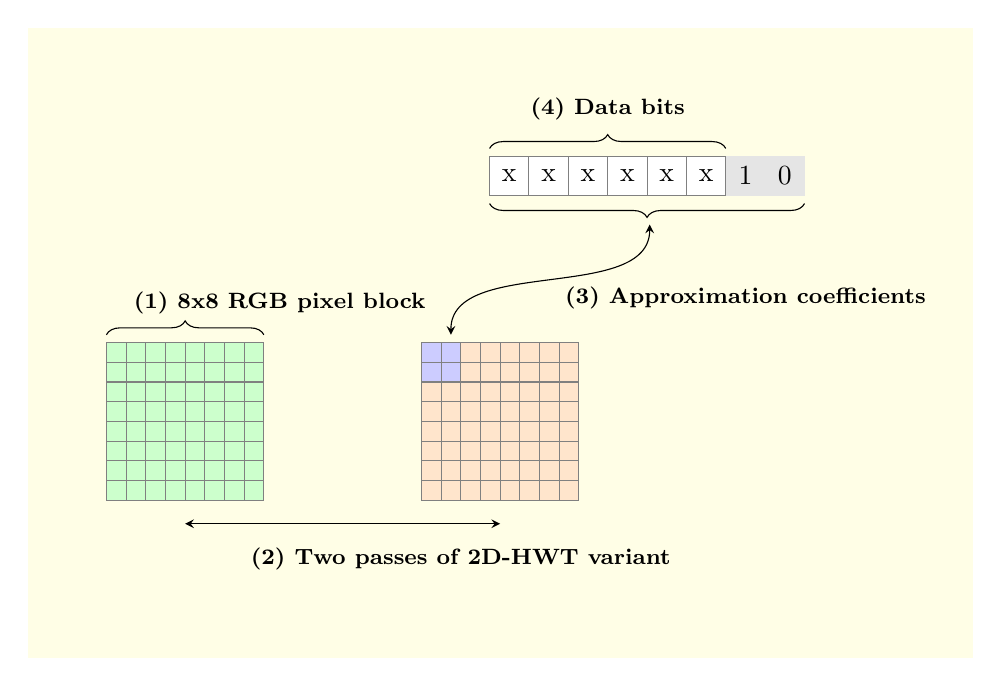
\begin{tikzpicture}[]


% bg bg

\fill[fill = yellow!10] (-2,-2) rectangle (10,6);

% bg
\fill[fill = green!20] (-1,0) rectangle (1,2);

\fill[fill = orange!20] (3-0.0001,0) rectangle (5,2);
\fill[fill = blue!20] (3-0.0001,1.5) rectangle (3.5,2);


% grids
\draw[step=0.25,color=black!50!white] (-1,0) grid (1,2);
\draw[step=0.25,color=black!50!white] (3-0.0001,0) grid (5,2);

% bits
\fill[xshift=110, yshift=110, fill = white] (3,0) (0,0) rectangle (4,0.5);
\draw[xshift=110, yshift=110, step=0.5,color=black!50!white, fill=white] (0,0) grid (4,0.5);



\draw[xshift=110, yshift=110] node at (0.25,0.25) {x};
\draw[xshift=110, yshift=110] node at (0.75,0.25) {x};
\draw[xshift=110, yshift=110] node at (1.25,0.25) {x};
\draw[xshift=110, yshift=110] node at (1.75,0.25) {x};
\draw[xshift=110, yshift=110] node at (2.25,0.25) {x};
\draw[xshift=110, yshift=110] node at (2.75,0.25) {x};

\draw [decorate,decoration={brace,amplitude=5pt}]
   (-1,2.1) -- (1,2.1);
\draw [decorate,decoration={brace,amplitude=5pt},xshift=110, yshift=110]
   (0,0.6) -- (3,0.6);
\draw [decorate,decoration={brace,amplitude=5pt},xshift=110, yshift=110]
   (4,-0.1) -- (0,-0.1);

\fill[xshift=110, yshift=110, fill = black!10!white] (3,0) rectangle (4,0.5);

\draw[xshift=110, yshift=110] node at (3.25,0.25) {1};
\draw[xshift=110, yshift=110] node at (3.75,0.25) {0};


% arrows

\draw[font={\footnotesize \bfseries}] node at (1.2,2.5) {(1) 8x8 RGB pixel block};


\draw[<->,>=stealth] (0,-0.3) -- (4,-0.3);
\draw[font={\footnotesize \bfseries}] node at (3.5,-0.75) {(2) Two passes of 2D-HWT variant};

\draw[<->,>=stealth] (3.375,2.1) .. controls (3.375,3.1) and (5.9,2.5) .. (5.9,3.5);
\draw[xshift=110, yshift=110, font={\footnotesize \bfseries}] node at (3.25,-1.3) {(3) Approximation coefficients};

\draw[xshift=110, yshift=110, font={\footnotesize \bfseries}] node at (1.5,1.1) {(4) Data bits};


\end{tikzpicture}
    
    \caption{Outline of the encoding process}
    \label{tikz:haar}
\end{center}
\end{figure}

The CImg class does contain Haar transforms but these are not suitable. We require an integer lifting scheme (described in \cite{XXX}) to ensure that the transform is reversible (without information loss). In the 1-dimensional case, for a pair of approximation and difference coefficients $(c_a,c_d)$, we calculate the output value pair $(x,y)$: 

\begin{eqnarray}
    x = & c_a + \lfloor \frac{c_d+1}{2} \rfloor \nonumber \\ 
    y = & x - c_d
\end{eqnarray}

Iteration of the above over pairs in both vertical and horizontal axis can be used to perform the full 2D HWT and its inversion losslessly.

Changing the approximation coefficients can also lead to capping of values as they are mapped back to greyscale space, outside the 0-255 range. We therefore selectively discard high frequency information (during the inverse transform) from the difference coefficient $c_d$ whenever capping occurs - leaving the approximation coefficients intact and the output within range. See appendix XXX for full details of the exact HWT variant used.


\FloatBarrier
\subsection{N-bit scaling}

The base class {\tt ScaledConduitImage} contains functions to code n-bits of data to and from a single pixel. The value of n is set on instancaition.

Two subclasses are specified for $n=3$ and $n=4$. For $n=3$ we use 3x2 blocks of pixels with a block size of 3-bytes. For $n=4$ we use blocks of 2 pixels with a block size of 1-byte.

The scaling process works so that the intervals for each data point are of equal width, except for the intervals at either end which are $\frac{1}{2}$ length. This is because extreme values (0 or 255) can only be either decreased or increased due to compression artifacts, not both. An input pixel value of 255 might result in 254 or 253 after compression, but never 0 or 1.


\FloatBarrier
\section{Testing}
    \begin{itemize}
        \item Unit
        \item Regression
        \item Black box
        \item White box
        \item Integration
        \item Security/penetration testing?
    \end{itemize}
    
    Security tests
    
    \begin{itemize}
    
    \item Use of the eval() and secureEval() functions
    \begin{itemize}
        \item test secureEval(). Should only decode JSON objects. Should only do so from Facbook API requests.
    \end{itemize}
    
    \item Insertion of text in to page. Easy since we can use JavaScript and RegExp.
    \begin{itemize}
        \item We allow all uppercase lowercase letters and numerals. Also allow .,?!(). That's it, better safe than sorry. Means no linking to malicious pages. Fully test all boundary cases etc etc.
    \end{itemize}
    
    \item UTF-decoder. Slightly harder since have to look at bytes not characters. Using the following rules we conformance test, test all boundaries etc etc. Put list of test inputs in appendix.
    \begin{itemize}
        \item We accept any valid, non-overlong, UTF8 byte sequences, max length 4-bytes, with scalar value:
        \begin{itemize}
            \item 0xB0 - 0xD7FF
            \item 0xE000 - 0x100AF
            \item 0x1B000 - 0x1BFFE (would-be surrogate pairs)
            \item 0x10F0000 (indicates a padding byte was added, only one allowed per decode)
        \end{itemize}
        \item We therefore must throw an exception whenever a valid UTF8 byte sequence is presented with scalar value:
        \begin{itemize}
            \item 0x0 - 0xAF (out of range)
            \item 0xD800 - 0xDFFF (surrogate pair characters)
            \item 0x100B0 - 0x1AFFF (out of range)
            \item 0x1BFFF - 0x10EFFFF (out of range)
            \item 0x10F001 - 0x1FFFFF (out of range)
        \end{itemize}
        \item We also throw and exception for valid UTF8 sequences when:
        \begin{itemize}
            \item They have an overlong form i.e. the same scalar value can be represented using a shorter byte sequence.
            \item They have scalar value 0x10F0000 (padding character) but this has already been seen during decoding.
            \item They have scalar value 0x10F0000 (padding character) but the final decoded byte sequence (before padding removal) has length less than 2.
            \item The final decoded byte sequence has length less than 1.
            \item They are longer than 4-bytes.
        \end{itemize}
        \item Naturally we reject any (invalid) UTF8 byte sequences with:
        \begin{itemize}
            \item Unexpected continuation bytes when we expect a start character.
            \item A start character which is not followed by the appropriate amount of valid continuation bytes - including start characters right at the end of a sequence.
        \end{itemize}
            
    \end{itemize}
    
    \item Public key downloader. Simply limit size, don't use exact size since other implementation might use different key sizes.
    
    \end{itemize}
    
    
    

